\documentclass[twoside,twocolumn,openright]{article}

\usepackage[papersize={8.5in, 11.393in},outer=6cm]{geometry} % magazine "standard size", source : http://momentumpress.com/sccc/LD/Resources/MagazinePageSize.pdf
\usepackage[T2A,T1]{fontenc}
\usepackage[utf8]{inputenc}
\usepackage[russian,english]{babel}
\usepackage{wrapfig}
\usepackage{graphicx}
\usepackage{lettrine}
\usepackage{lipsum}
\usepackage[usenames,dvipsnames,svgnames,x11names,table]{xcolor}
\usepackage{microtype}
\usepackage[colorlinks=true,linkcolor=blue,citecolor=blue]{hyperref}
\usepackage[defaultmono, scale=.90]{droidsansmono}
\usepackage{eso-pic}
\usepackage{tikz}


\tikzset{
  every overlay node/.style={
    draw=black,fill=white,rounded corners,anchor=north west,
  },
}
% Usage:
% \tikzoverlay at (-1cm,-5cm) {content};
% or
% \tikzoverlay[text width=5cm] at (-1cm,-5cm) {content};
\def\tikzoverlay{%
   \tikz[baseline,overlay]\node[every overlay node]
}%


\usepackage{fancyhdr}
\setlength{\headheight}{15.2pt}
\fancyhf{}
\fancyhead[C]{\thepage}
\renewcommand{\headrulewidth}{0pt}
\pagestyle{fancy}
%\setcounter{page}{1}

\begin{document}


\AddToShipoutPictureFG*{\put(0,0){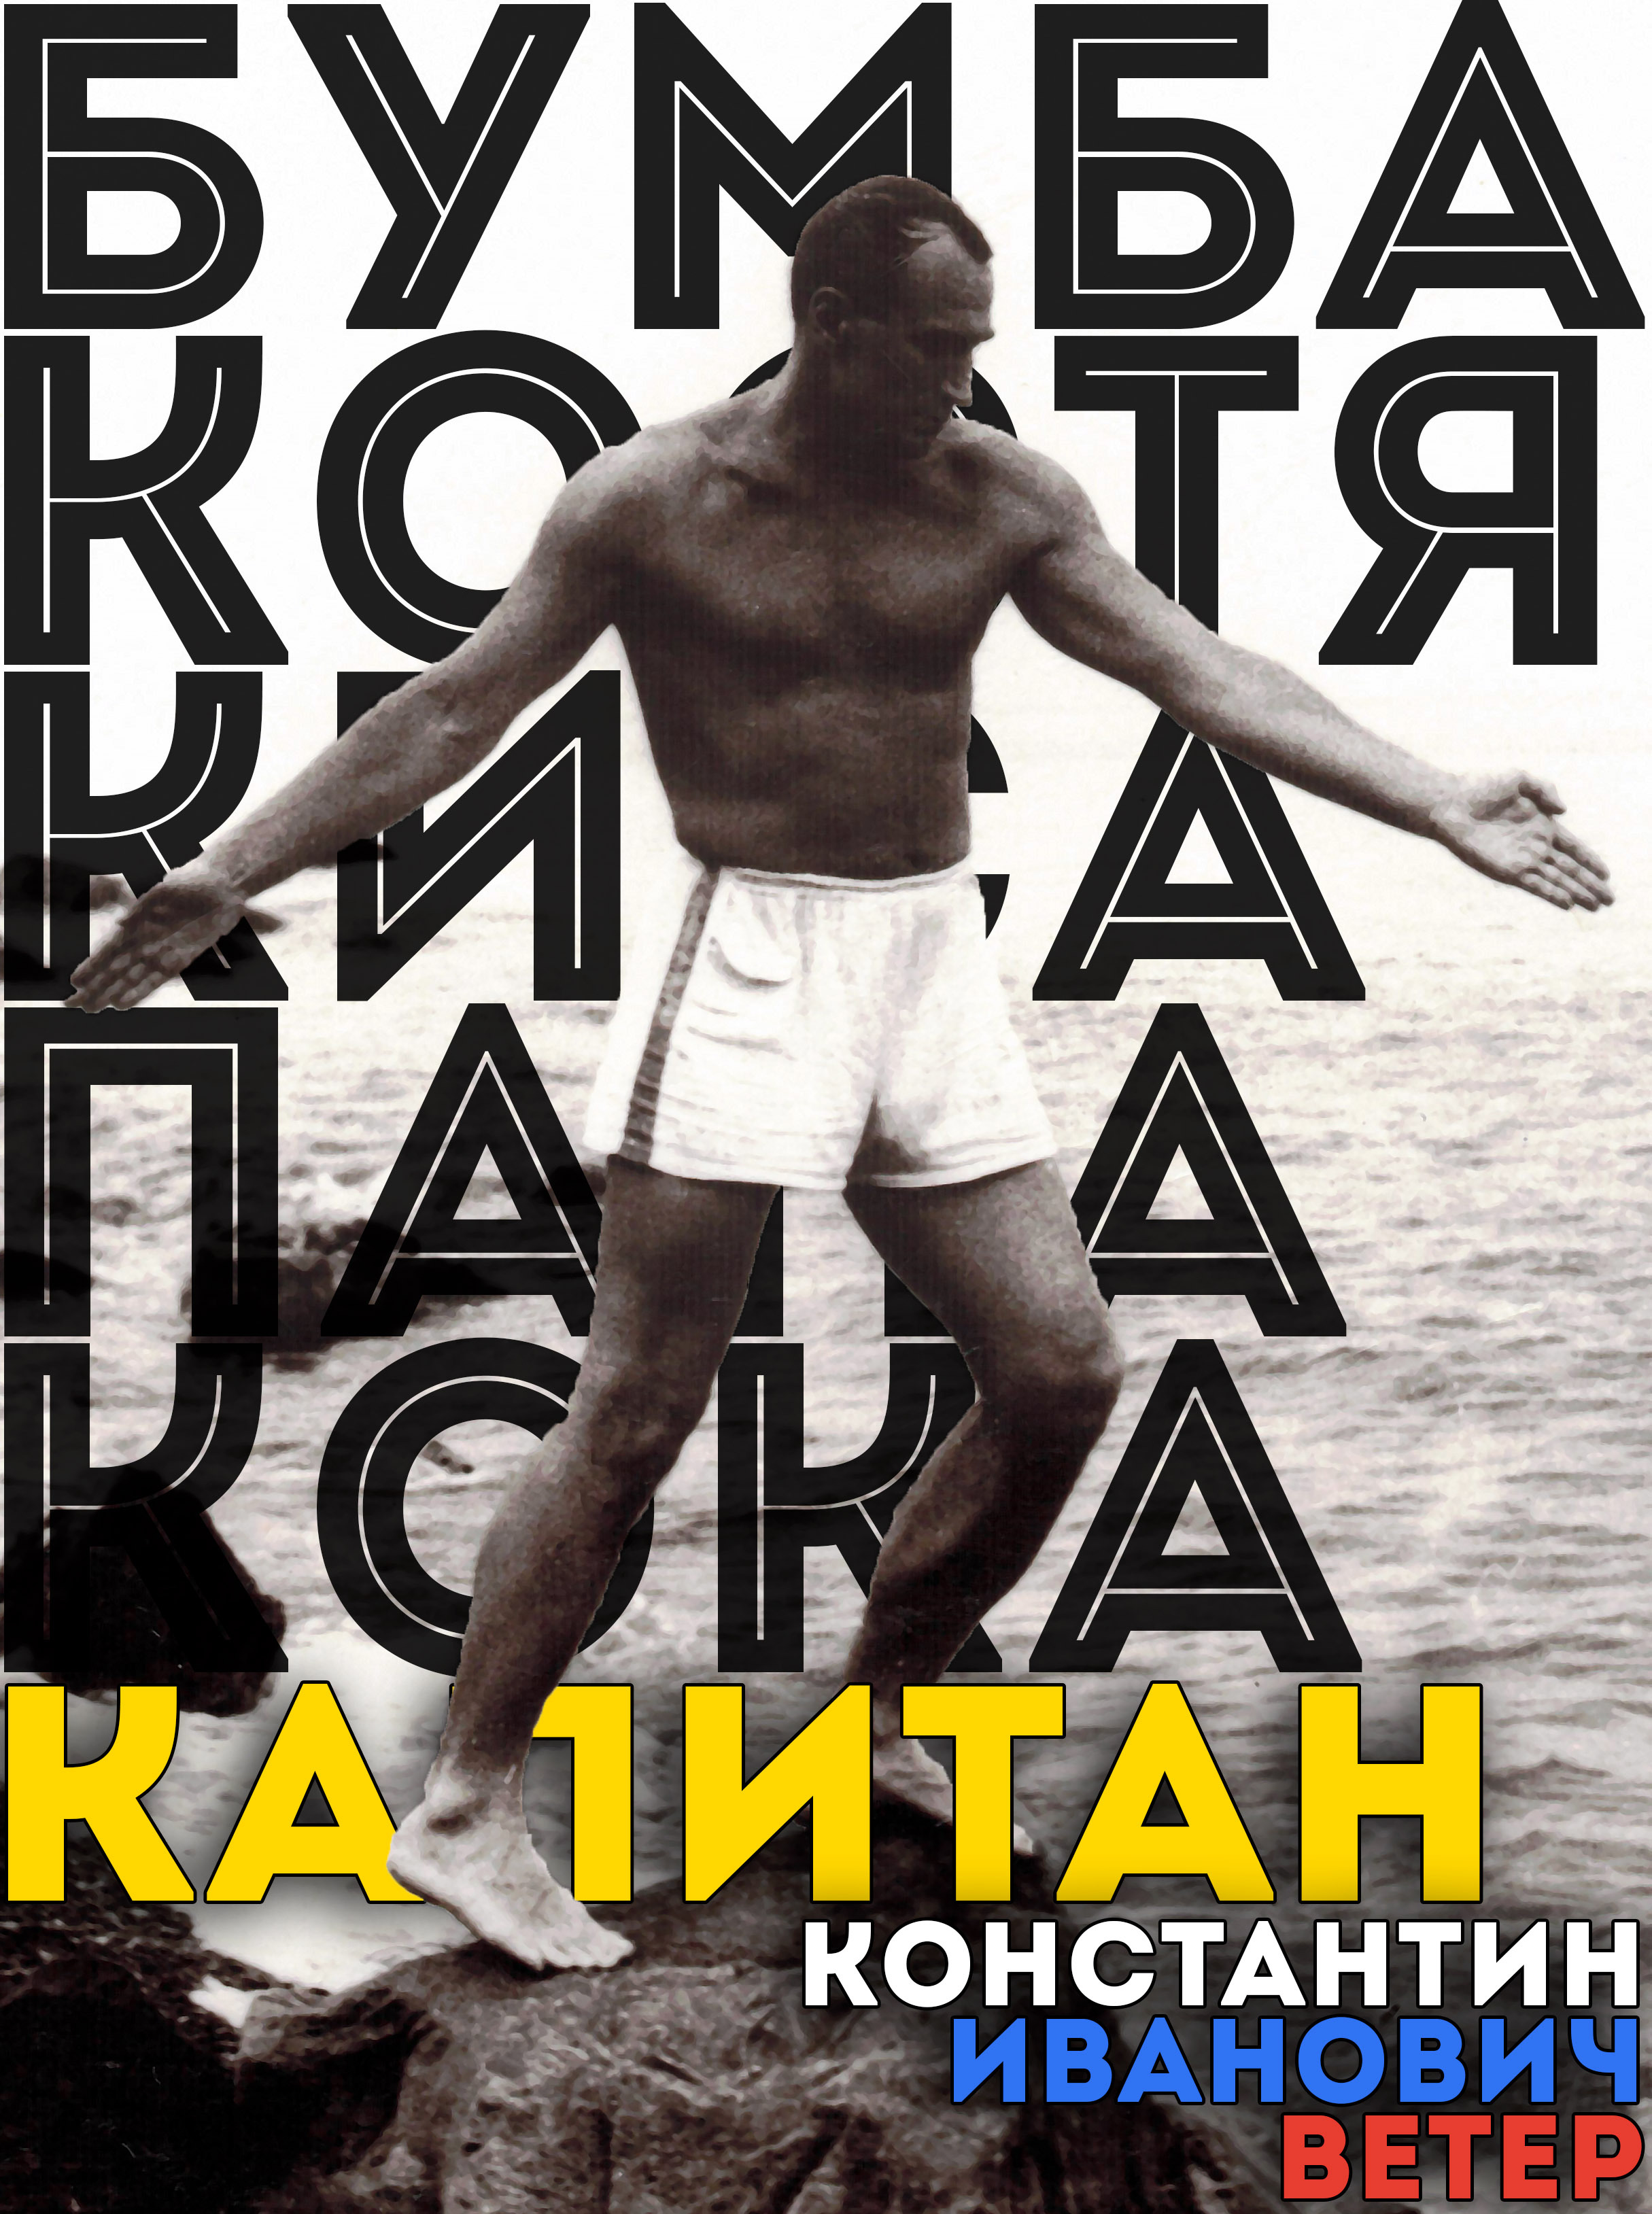
\includegraphics[width=8.5in,scale=1]{img/ocean_gpa_cover_short.jpg}}}
.\newpage.\newpage

\lettrine[lines=2]{Y}{esterday} morning at 5:30 AM my grandfather died. 
\\\\
We were close. Closer, I dare say, than most. My own having father passed when I was very young, Grandpa Kostia – or Bymba, as I first called him – quickly assumed the mantle of my raising. Of any single individual he plausibly had the greatest influence on my childhood development, both through his direct mentorship as well as more indirectly, in the capacity of role model. I spent many thousands of hours in his company, on walks through the woods and deserts, tending the plants of our dacha, swimming in backcountry lakes and overchlorinated pools, looking at the stars and the moon’s craters and the conjunctions of planets. He took me on cross-country trips, on overnight train rides to distant cities, through squares and museums and space centers. Calling upon half-borrowed connections, he clad me in scuba gear and chucked me into the pool at the Gagarin Training Center while hopeful cosmonauts practiced EVAs. In the motherland he was at home, and exerted himself in the service of my betterment.
\\\\
In even more distant lands and distant straits, he’d wait patiently for untold hours as I read through lengthy book series while lounging on grocery store patio furniture, or else stand around browsing utterly uninteresting electronics as I played video game demos. He developed many structured activities for us to do, scavenging old wood and canvas from dumpsters to build sailboats and hang gliders, hiding the disarticulated “skeletons” of “baby dinosaurs” for me to find in the miles of land surrounding our home, undertaking ill-conceived supplemental feeding campaigns for local insect populations, and hurling objects of myriad shapes and sizes back and forth across long distances separated by open fields. His more explicit lessons were sometimes strange – when beset by attackers, the eyes, groin, and throat make the most vulnerable targets – but those were easily filed away in the uncomfortable hope of never having to be used. We played thousands of seated games, of chess and checkers, dominoes and go, and favorite of all – the fool, which I left him more often than not. All together, we threw perhaps a million darts and basketballs, pinkies and rocks. Neither of us was ever very good. 
\\\\
Until his mid-seventies I thought him in excellent health. One summer in Phoenix, AZ, I took him on a quick midday hike up a local mountain along an exceptionally steep and scrambly “trail” that, in retrospect, I may have invented of whole cloth. As we neared the top, I noticed him swaying slightly, and breathing not through his nose but through his open mouth! Where was the man who’d so effortlessly fling me through the air, who’d happily brave with me and my unfortunate, un-consenting baby brother (in rickety push stroller) the 50C heat as we fetched groceries, who’d toss boomerangs in unshaded fields, sustain first degree burns on scorching playground equipment, and search for quarters on the streets that we might buy cold, refreshing carbonated beverages from discount vending machines? The vicissitudes of age were uncompromising indeed.

\tikzoverlay[text width=7in] at (-1.9in,6.65in) {
  \LARGE{The Seven Lives of \textcolor{DarkRed}{Konstantin Vetr}}
};

Before easy telecommunications arrived, we were unable to interact much during times apart. But Bymba nevertheless made do, sending me many dozens of letters inquiring after and commenting on my own affairs, describing his comings and goings throughout Russia, and always including some sort of hand-drawn puzzle for me to solve, often requiring the application of both verbal and mathematical reasoning.
\\\\
But by my mid-teens cell phones had grown commonplace, so we were able to maintain a regular telephone habit after I’d departed from hearth and home. Almost every morning on my walk into school or work, I’d give him and grandma a call. He’d rarely pick up, but she usually would, if on the second or third attempt, and hand the phone over after we finished speaking ourselves. For want of deeper conversation, I eventually happened upon a most devious strategy: a relentless bullying campaign replete with provocation, shame, and harassment. Over the last decade I imported and forced him to read many dozens of books – mostly translations of Western pop-sci, history, philosophy, and fiction I'd grown up reading – and then pirated \& photo-copied, enlarged, and printed out dozens more for him to read after his vision began to fade. During those morning chats and after not inconsiderable nagging, I’d extract from him a book report on the initially 10-20 but eventually 1-2 pages he'd read the day before, and we’d discuss its finer points in detail. The fiction was rarely to his liking (Sagan’s Contact being the rare exception, though Robinson's Mars trilogy and Weir’s Martian were also tolerable), but he certainly enjoyed the non-fiction, breathlessly recounting “new” insights from cosmology, genetics, astrophysics, paleontology, and other disciplines. At times, we’d deviate from this pattern, substituting reading homework with e.g. 3-D puzzle homework, but by and large we were able to get through several dozen works from almost just as many authors and topics.
\\\\
I was unfortunately unable to reach him in his final moments – the phone call arrived just as I was packing to leave for a morning flight out, and his death was sudden enough that my request for updates on his condition, that I might drive or fly out sooner, went unfulfilled. But outside some sort of peak-end bias, I’m not sure it’s quite right to privilege certain person-moments over others. If anything, later moments seem of lower priority for their inability to psychologically influence whatever succeeds them. Bymba was a proud man, and likely would not have wanted to be seen in the condition that characterized his passing. That said… I’d have wanted nothing more than to hold his hand, reading papers, writing code, and taking meetings from his bedside. Instead, our last interactions were some weeks prior, at such time as he could still shuffle about the house and yard. He gifted me a watch that he’d received from his friend Georgy Beregovoy many decades ago, a Raketa World Time, and we went through all the cities listed on the bezel and recounted to each other our respective experiences in each. We played several games of chess, cards, and dominos, almost evenly matched. We ate together and enjoyed one another’s company. I’m sorry I couldn’t be with you in the end, Bymba, but I hope our last moments together were enough.
\\\\
(if anything, we’re now even, you having missed my own birth by months while off on some sailing adventure. For just as with your exit, I came into this world prematurely)
\\\\
Surprisingly, Bymba also existed prior to my birth. Over those sixty-some years, his accomplishments were many, enough to fill several lifetimes. He was a sailor, sportsman, \& storyteller, a cosmonaut \& steadfast companion, an engineer \& trickster. He designed rocket boosters and atmospheric reentry capsules, spent thousands of hours training for missions alongside or under his friends Kamanin, Gagarin, and Korolev, and sailed across many seas and oceans, both as part of a larger crew and alone. He was a Master of Sport in yachting and skydiving, setting many records across 2,000+ jumps. In boxing and cross-country skiing, he merely competed in the Second-Class, and could also perform many impressive feats of athleticism, such as 45 consecutive non-kipping pull-ups. Even unto his eventual confinement in bed and subsequent death, he continued to do his daily exercises, though they eventually dwindled from the hoisting of makeshift atlas stones to the pressing of lightweight dumbbells. Always a bit of a peacock, he enjoyed having his feathers preened by my advertisement via interviews and photos on websites such as Reddit. And as with every woman aged 18-80 to cross his path, he often flirted with other vocations, spending years driving tanks and diesel-powered submarines, playing the piano and guitar, and illegally building personal transportation vehicles ranging from hot air balloons to helicopters. Between these, Nazi occupation, and exposure to radiation not far from the Chernobyl exclusion zone, it’s truly a wonder he did not die sooner.
\\\\
He loved to play pranks on his family and friends, and was a consummate cheat in games of chance and skill, though always in good fun, and always fessing up moments after his ill-earned victories. We’d get him back, in turn: a favorite childhood pastime of mine was watching him return to our apartment building laden heavily with groceries. After ringing him in, I’d rush to our floor’s lobby and quickly summon both elevators. In exchange for sending them to the top floor and resummoning them to our own a dozen times, I’d be rewarded by grandpa’s strained face emerging from the stairwell. Any lack of consideration for other building residents I rest entirely on his shoulders. And while not many still live with distinct memories of his deeds and misdeeds – the children of his colleagues and friends long dead from old age – several of them were compiled into an autobiographical memoir he wrote decades ago, featuring, as I’ve gathered, only the usual amounts of exaggeration and embellishment.
\\\\
Of these and many other faults, Bymba, you also aspired quite strongly towards hypocrisy. Nothing but the strongest, blackest of coffees and teas for me, you’d proclaim, while happily mixing yourself a sugar-laden, coffee-flavored milkshake. Never has a drop of alcohol nor tobacco fume has entered my mouth! you’d announce while sipping from a glass of wine and smoking your yearly cigar. Soda is evil incarnate, quenching no thirst and rotting not only teeth but mind as well, you’d advise while purchasing our hundredth Big Gulp that year, to sit outside the gas station and play with me some bastardization of curling with scattered pebbles. Gambling, what a terrible sin; but do take these arcade tokens and booster packs, I’ve bought them for you. The spirit of adventure, how invigorating and thrilling! Yet you’d wait up until the wee hours for me to return from any overlong “day-hikes” or cross-country road trips, and how you fretted when I first began solo-backpacking in my mid-teens. I’m sorry for worrying you.
\\\\
At the end of every conversation, you would always promise the following: to always remember me, to always love me, and to always wait for me. It would appear that you have failed to keep this promise. I feel I cannot quite promise in return, for sheer physical impossibility, if nothing else. But while I don’t think there’s much left to wait for, remembrance and love of the man who raised me are two faculties as yet within my power. It’s not much, but it will have to do.



\end{document}